


% https://tex.stackexchange.com/questions/7208/how-to-vertically-center-the-text-of-the-cells
% https://stackoverflow.com/questions/25163873/horizontal-and-vertical-alignment-in-tabular-cell
\begin{table}[th]
    \centering
    \caption[Slowly synchronizing and sync-maximal $n$-state automata]{Slowly synchronizing and sync-maximal automata. 
    	Names from the literature and reset lengths are indicated. 
    	The marked state is used to deduce sync-maximality via \THM~\ref{sync_max:thm:circular_sync_max} in the proof of \THM~\ref{sync_max:thm:families}.
    	%Additionally, every primitive group
    	%together with a non-permutation of rank $n - 1$ yields such extremal automata for the set of synchronizing words~\cite{zweiarbeiten.}.
    } 
 \begin{tabular}{c|c|c|c}%p{2.2cm}} 
 \hline 
  Name & Automata & Reset Length & Referenz \\ \hline
  $\mathcal C_n$ & 
  \begin{tabular}{l}
   \rule[-0.02cm]{0pt}{2.15cm}
 \scalebox{.8}{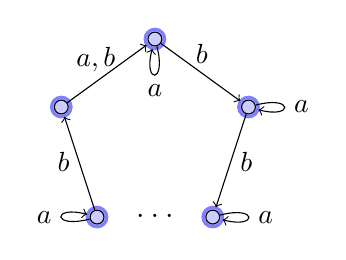
\begin{tikzpicture}[shorten >=1pt,->,node distance=4cm]
  %\tikzstyle{vertex}=[circle,color=red!60,fill=black!10,minimum size=25pt,inner sep=1pt,very thick]
  \tikzstyle{vertex}=[circle,draw,minimum size=5pt,inner sep=1pt]
 
  \foreach \name/\angle/\text in {P-n-2/234/n-2, P-n-1/162/n-1, 
                                  P-0/90/0, P-1/18/1, P-2/-54/2}
{
	\ifthenelse{\equal{\angle}{162}}
	{
		\node[circle,draw,minimum size=7pt,inner sep=1pt,draw=blue!50,very thick,fill=blue!20] (\name) at (\angle:1.25cm) {};
	}
	{
		\node[vertex] (\name) at (\angle:1.25cm) {};
	}
}

  % \node at (0, -1.5) {$\ldots$};

   \path[->] (P-n-2) edge [left] node {$b$} (P-n-1);
   \path[->] (P-n-1) edge [above,pos=0.35] node {$a,b$} (P-0);
   \path[->] (P-0) edge [above] node {$b$} (P-1);
   \path[->] (P-1) edge [right] node {$b$} (P-2);
   
   \path[->] (P-n-2) edge [loop left] node {$a$} (P-n-2);
   \path[->] (P-0) edge [loop below] node {$a$} (P-0);
   \path[->] (P-1) edge [loop right] node {$a$} (P-1);
   \path[->] (P-2) edge [loop right] node {$a$} (P-2);
   
  \node at (0, -1) {\large $\ldots$};
\end{tikzpicture}}%
\end{tabular} & $(n-1)^2$ & %Transforms to $\mathcal W_n$ with $b$ and $c = ab$,
\cite{AnaVolGus2013,Cer64,DBLP:journals/ijfcs/Maslennikova19} \\  \hline
\begin{tabular}{l} 
$\mathcal V_n = \mathcal W_n$ 
\end{tabular}
& 
\begin{tabular}{l} 
 \rule[-0.02cm]{0pt}{2.15cm}
 \scalebox{.8}{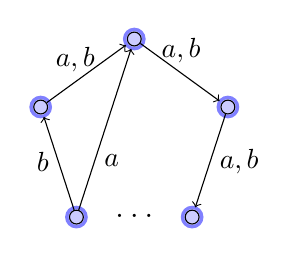
\begin{tikzpicture}[shorten >=1pt,->,node distance=5cm]
  \tikzstyle{vertex}=[circle,draw,minimum size=5pt,inner sep=1pt]
 
  \foreach \name/\angle/\text in {P-n-2/234/n-2, P-n-1/162/n-1, 
                                  P-0/90/0, P-1/18/1, P-2/-54/2}
{
	\ifthenelse{\equal{\angle}{234}}
	{
		\node[circle,draw,minimum size=7pt,inner sep=1pt,draw=blue!50,very thick,fill=blue!20] (\name) at (\angle:1.25cm) {};
	}
	{
		\node[vertex] (\name) at (\angle:1.25cm) {};
	}
}
   
  % \node at (0, -1.5) {$\ldots$};

  \path[->] (P-n-2) edge [left] node {$b$} (P-n-1);
  \path[->] (P-n-1) edge [above,pos=0.35] node {$a,b$} (P-0);
  \path[->] (P-0) edge [above] node {$a,b$} (P-1);
  \path[->] (P-1) edge [right] node {$a,b$} (P-2);
   
  \path[->] (P-n-2) edge [right,pos=0.3] node {$a$} (P-0);
   
  \node at (0, -1) {\large $\ldots$};
\end{tikzpicture}} 
\end{tabular}
& 
\begin{tabular}{l} $n^2 - 3n + 3$ 
\end{tabular}
& \cite{AnaVolGus2013,DBLP:journals/ijfcs/Maslennikova19}
\\ \hline 
  \begin{tabular}{l}
  $\mathcal L_n = \mathcal D_n'$
  \end{tabular} 
 &
  \begin{tabular}{l} 
   \rule[-0.02cm]{0pt}{2.15cm}
       \scalebox{.8}{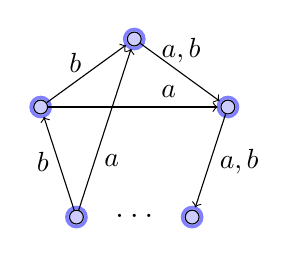
\begin{tikzpicture}[shorten >=1pt,->,node distance=4cm]
  \tikzstyle{vertex}=[circle,draw,minimum size=5pt,inner sep=1pt]
 
  \foreach \name/\angle/\text in {P-n-2/234/n-2, P-n-1/162/n-1, 
                                  P-0/90/0, P-1/18/1, P-2/-54/2}
{
	\ifthenelse{\equal{\angle}{162}}
	{
		\node[circle,draw,minimum size=7pt,inner sep=1pt,draw=blue!50,very thick,fill=blue!20] (\name) at (\angle:1.25cm) {};
	}
	{
		\node[vertex] (\name) at (\angle:1.25cm) {};
	}
}
   
   %\node at (0, -1.5) {$\ldots$};

   \path[->] (P-n-2) edge [left] node {$b$} (P-n-1);
   \path[->] (P-n-1) edge [above,pos=0.35] node {$b$} (P-0);
   \path[->] (P-0) edge [above] node {$a,b$} (P-1);
   \path[->] (P-1) edge [right] node {$a,b$} (P-2);
   
   \path[->] (P-n-2) edge [right,pos=0.3] node {$a$} (P-0);
   \path[->] (P-n-1) edge [above,pos=0.7] node {$a$} (P-1);
   
  \node at (0, -1) {\large $\ldots$};
\end{tikzpicture}}
  \end{tabular}
    & $n^2 - 3n + 4$ & \cite{AnaVolGus2013,DBLP:journals/ijfcs/Maslennikova19}   \\ \hline
\begin{tabular}{l}
$\mathcal F_n$ \\ 
$n > 3$ odd  
\end{tabular} &

\begin{tabular}{l}
 \rule[-0.02cm]{0pt}{2.15cm}
 \scalebox{.8}{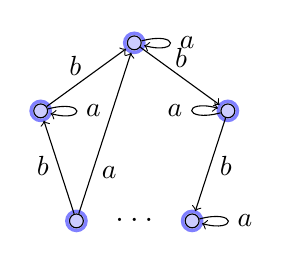
\begin{tikzpicture}[shorten >=1pt,->,node distance=5cm]
  %\tikzstyle{vertex}=[circle,color=red!60,fill=black!10,minimum size=25pt,inner sep=1pt,very thick]
  \tikzstyle{vertex}=[circle,draw,minimum size=5pt,inner sep=1pt]
 
  \foreach \name/\angle/\text in {P-n-2/234/n-2, P-n-1/162/n-1, 
                                  P-0/90/0, P-1/18/1, P-2/-54/2}
{
	\ifthenelse{\equal{\angle}{234}}
	{
		\node[circle,draw,minimum size=7pt,inner sep=1pt,draw=blue!50,very thick,fill=blue!20] (\name) at (\angle:1.25cm) {};
	}
	{
		\node[vertex] (\name) at (\angle:1.25cm) {};
	}
}

   \path[->] (P-n-2) edge [left] node {$b$} (P-n-1);
   \path[->] (P-n-1) edge [above,pos=0.35] node {$b$} (P-0);
   \path[->] (P-0) edge [above] node {$b$} (P-1);
   \path[->] (P-1) edge [right] node {$b$} (P-2);
   
   \path[->] (P-n-2) edge [right,pos=0.25] node {$a$} (P-0);
   \path[->] (P-n-1) edge [loop right] node {$a$} (P-n-1);
   \path[->] (P-0) edge [loop right] node {$a$} (P-0);
   \path[->] (P-1) edge [loop left] node {$a$} (P-1);
   \path[->] (P-2) edge [loop right] node {$a$} (P-2);
   \node at (0, -1) {\large $\ldots$};
\end{tikzpicture}}
\end{tabular}
& $n^2 - 3n + 3$ & \cite{AnaVolGus2013,DBLP:journals/ijfcs/Maslennikova19} \\ \hline
\begin{tabular}{l}
$\mathcal K_n = \mathcal G_n$ \\  $n > 5$ odd
\end{tabular}
 & 
\begin{tabular}{l}
 \rule[-0.02cm]{0pt}{2.15cm}
\scalebox{.8}{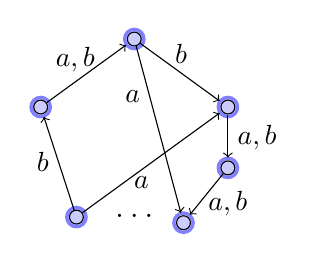
\begin{tikzpicture}[shorten >=1pt,->,node distance=5cm]
  \tikzstyle{vertex}=[circle,draw,minimum size=5pt,inner sep=1pt]
 
  \foreach \name/\angle/\text in {P-n-2/234/n-2, P-n-1/162/n-1, 
                                  P-0/90/0, P-1/18/1, P-2/-18/2, P-3/-60/3}
{
	\ifthenelse{\equal{\angle}{90}}
	{
		\node[circle,draw,minimum size=7pt,inner sep=1pt,draw=blue!50,very thick,fill=blue!20] (\name) at (\angle:1.25cm) {};
	}
	{
		\node[vertex] (\name) at (\angle:1.25cm) {};
	}
}
   
   \node at (0, -1) {\large $\ldots$};

   \path[->] (P-n-2) edge [left] node {$b$} (P-n-1);
   \path[->] (P-n-1) edge [above,pos=0.35] node {$a,b$} (P-0);
   \path[->] (P-0) edge [above] node {$b$} (P-1);
   \path[->] (P-1) edge [right] node {$a,b$} (P-2);
   \path[->] (P-2) edge [right,pos=0.7] node {$a,b$} (P-3);
   
   \path[->] (P-n-2) edge [right,pos=0.3] node {$a$} (P-1);
   \path[->] (P-0) edge [left,pos=0.3] node {$a$} (P-3);
\end{tikzpicture}}
\end{tabular}
& $n^2 - 4n + 7$ & \begin{tabular}{l} Thm.~\ref{sync_max:thm:families} \& \\ \cite{AnaVolGus2013,DBLP:journals/ijfcs/Maslennikova19} \end{tabular} \\ \hline
%- & Primitive Group + Rank $n - 1$ Non-Permutation & - & \cite{Hoffmann20}
\end{tabular}
    \label{def:Vn}\label{def:Ln}\label{def:Fn}\label{def:Kn}
    \label{tab:slowly_sync_families}
\end{table}

\todo[inline]{noch farblich makrieren wie in STACS paper} 